\section{Elektromagnetische Schwingungen und Wellen}
	
		\subsection{Der Schwingkreis}
		
		Zeichnung AB13.07.
		
		
		\textbf{Schaltung zur Auslösung einer freien gedämpften Schwingung}
		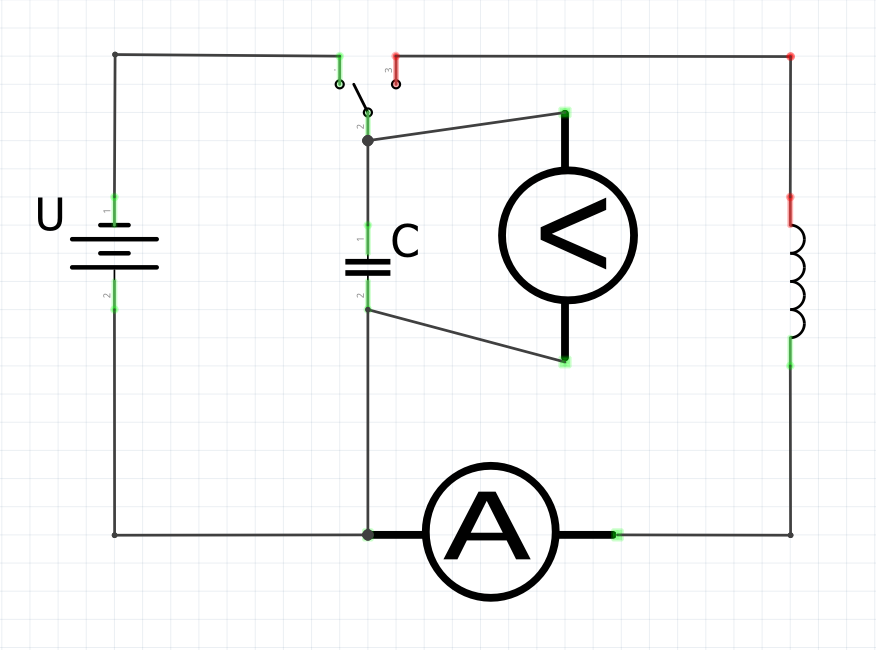
\includegraphics[scale=0.5]{Schwingkreis1}
			
			\subsubsection{Herleitung der physikalischen Gesetze des Schwingkreises}
			
			\begin{itemize}
				\item Wdh. mech. Schwingung: \\
					Kraftgesetz: Die Federkraft ist der Elongation s proportional: \\
					$ \Rightarrow F_R = -D \ast s $ \\
					Kräftegleichung: \\
					$ m \ast a_{(t)} = -D \ast s_{(t)} $ \\
					Differentialgleichung: \\
					$ m \ast \ddot{s}_{(t)} = -D \ast s_{(t)} $ \\
					$ \ddot{s}_{(t)} = -\frac{D}{m} \ast s_{(t)} $ \\
					Lösungsfunktion: $ s_{(t)} = \hat{s} \ast sin(\omega \ast t) $ \\
					\hspace{24mm} mit $ \omega = \sqrt{\frac{D}{m}} $
					
				\item Analog im elektromagnetischen Fall: \\
					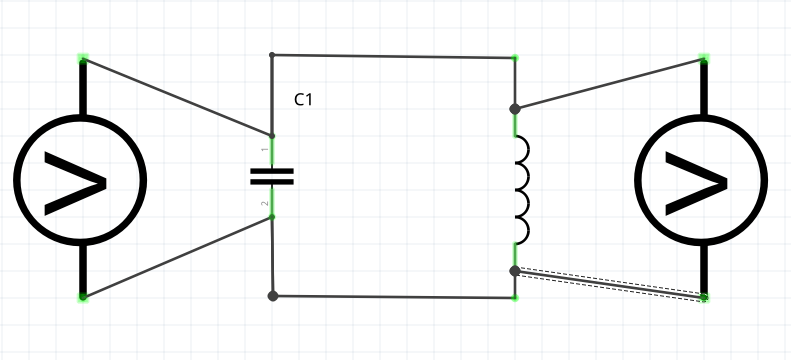
\includegraphics[scale=0.4]{Schwingkreis2} \\
					$ U_{C_{(t)}} = \frac{Q_{(t)}}{C}$ \hspace{21mm}Links \\
					$ U_{ind_{(t)}} = -L \ast \dot{I}_{(t)} $ \hspace{10mm}Rechts \\
					Spannungsgleichung: \\
					$ U_{C_{(t)}} = U_{ind_{(t)}} $ \\
					$ \frac{Q_{(t)}}{C} = -L \ast \dot{I}_{(t)} $ \\
					Differentialgleichung: \\
					$ \dot{I}_{(t)} = -\frac{1}{L \ast C} \ast Q_{t} $ \\
					$ \ddot{Q}_{(t)} = -\frac{1}{L \ast C} \ast Q_{(t)} $ \\
					$ Q_{(t)} = \hat{Q} \ast sin(\omega \ast t + \varphi) $ \\
					mit $ \omega = \sqrt{\frac{1}{L \ast C}} $ \\
			\end{itemize}
			
			\subsubsection{Merke:}
			
			Aus der Spannungsgleichung erhält man im elektromagnetischen Schwingkreis $ \omega = \sqrt{\frac{1}{L \ast C}} $ und $ T = \frac{2\pi}{\omega} = \frac{2\pi}{\sqrt{\frac{1}{L \ast C}}} = 2\pi \ast \sqrt{L \ast C}$ (thomson'sche Schwingungsgleichung)